\chapter{Considerações Gerais}
\label{cap:02}

\textbf{Texto das considerações gerais, dividido em subseções}

% Este é um exemplo de como usar figuras. Referência cruzada: Figura~\ref{fig:exemplo}

% \FloatBarrier
% \begin{figure}[!htbp]
% 	\centering
% 	\caption{Exemplo de figura}
% 	%scale redimensiona a figura.
% 	%1.5 = 150% do tamanho original
% 	%1 = 100% do tamanho original
% 	%0.20 = 20% do tamanho original
% 	
\includegraphics[scale=0.4]{imagens/exemploFigura}
% 	\\\textbf{Fonte:} Elaborada pelo autor
% 	\label{fig:exemplo}
% \end{figure}
% \FloatBarrier

% Este é um exemplo de como usar equações. Referência cruzada: Equação~\ref{eq:exemplo}

% \begin{equation}
% \sum_{i=1}^{n} i = \frac{n(n+1)}{2}
% \label{eq:exemplo}
% \end{equation}
%
%

% Exemplo de inserção de lista de código fonte:

% \lstinputlisting[language=Java]{fontes/ClasseExemplo.java}

% Este é um exemplo de como inserir texto sem formatação (ambiente verbatim):

% \begin{verbatim}
% Texto sem formatação, como espaçamento igual.
% \end{verbatim}

% Exemplos de comandos para texto e referências:

% \begin{itemize}
% 	\item Para iniciar um novo parágrafo, basta deixar uma linha em branco no código fonte;
% 	\item Não force o compilador a pular mais de uma linha, pois terá influência negativa na composição do documento;
% 	\item Sempre deixe o \LaTeX\ realizar a formatação de parágrafos e posicionamento de elementos;
% 	\item Utilização de aspas simples (abertura \verb|`|, fechamento \verb|'|): `Texto entre aspas simples';
% 	\item Utilização de aspas duplas (abertura \verb|``|, fechamento \verb|''|): ``Texto entre aspas duplas'';
% 	\item Negrito (comando \verb|\textbf|): \textbf{texto em negrito};
% 	\item Itálico (comando \verb|\textit|): \textit{texto em itálico};
% 	\item Sublinhado (comando \verb|\underline|): \underline{texto sublinhado};
% 	\item Negrito e itálico (usar comandos juntos): \textbf{\textit{texto em negrito e itálico}};
% 	\item Alterar cor do texto (comando \verb|\textcolor{cor}{texto}|):
% 	\begin{itemize}
% 		\item Exemplo \verb|\textcolor{red}{texto}|: \textcolor{red}{texto vermelho};
% 		\item Exemplo \verb|\textcolor[RGB]{255, 102, 0}|: \textcolor[RGB]{255, 102, 0}{texto laranja};
% 		\item Exemplo \verb|\textcolor[HTML]{006AD7}|: \textcolor[HTML]{006AD7}{texto azul};
% 	\end{itemize}
% 	\item Ambiente matemático inline (comando \verb|$ expressão $|): $s = x^2-2x +1$;
% 	\item Referência normal (comando \verb|\cite|):
% 	\begin{itemize}
% 		\item \cite{Agaisse1995};
% 		\item \cite{Abedi2014};
% 		\item \cite{BtNomenclature2016};
% 	\end{itemize}
% 	\item Referência normal com mais de uma obra (comando \verb|\cite|):
% 	\begin{itemize}
% 		\item \cite{Abedi2014, Agaisse1995};
%         \item \cite{AgapitoTenfen2014, BtNomenclature2016, Nelson2014};
% 	\end{itemize}
% 	\item Referência nome e ano (comando \verb|\citeauthorandyear|):
% 	\begin{itemize}
% 		\item \citeauthorandyear{Agaisse1995};
% 		\item \citeauthorandyear{Abedi2014};
% 		\item \citeauthorandyear{BtNomenclature2016};
% 	\end{itemize}
% \end{itemize}

% Exemplo 1 de citação direta:

% \begin{citacao}
% 	Os 20 aminoácidos usualmente encontrados como resíduos em proteínas contém um grupo $\alpha$-carboxil, um grupo $\alpha$-amino e um grupo R
% 	distinto substituído no átomo de carbono $\alpha$. O átomo de carbono $\alpha$ de todos os aminoácidos, com exceção da glicina, é assimétrico e,
% 	portanto, os aminoácidos podem existir em pelo menos duas formas estereoisoméricas. Somente os estereoisômeros L, com uma configuração relacionada à
% 	configuração absoluta da molécula de referência L-gliceraldeído, são encontrados em proteínas \cite[p. 81]{Nelson2014}.
% \end{citacao}

% Exemplo 2 de citação direta:

% \begin{citacao}
% 	\textit{These various insecticidal proteins are synthesized during the stationary phase and accumulate in the mother cell as a crystal inclusion
% 	which can account for up to 25\% of the dry weight of the sporulated cells. The amount of crystal protein produced by a B. thuringiensis culture in
% 	laboratory conditions (about 0.5 mg of protein per ml) and the size of the crystals (24) indicate that each cell has to synthesiz
% 	e $10^6$ to $2 \times 10^6$ $\delta$-endotoxin molecules during the stationary phase to form a crystal} \cite[p. 1]{Agaisse1995}.
% \end{citacao}

% Exemplo de nota de rodapé\footnote{Essa é uma nota de rodapé!}.

\section{Trabalhos Correlatos}

\textbf{Gophertype: Criação de um editor/aplicativo de treino de digitação em modo
texto (TUI) usando Go + Bubble Tea framework. \cite{Lindroos2025}}

\textbf{An Empirical Investigation of Command-Line Customization: Analisa mais de
2,2 milhões de aliases no GitHub e identifica padrões de personalização do shell:
atalhos, modificações e scripts \cite{SchroderCito2022}}

\textbf{On the design of text editors: analisa decisões implícitas em editores de
texto — como layout, tipografia, colorização e interações — e questiona se elas derivam
da falta de alternativas ou da repetição de hábitos entre desenvolvedores.
\cite{Rougier2020Editors}}

\section{Interface Modo Texto x Modo Gráfico}

Como os usuários interagiam com computadores antes das interfaces gráficas? Nos
primórdios da computação, programas e dados eram armazenados em cartões perfurados,
estes que eram pré-processados em lote e com longa espera de resultados. Com a constante
evolução das maquinas e a criação dos mainframes, grandes e poderosos
computadores que suportavam diversas interações simultaneamente e com níveis de
confiabilidade e multitarefa, fez com que a comunicação entre usuário e máquina passasse
a ser realizada de forma mais iterativa, principalmente por meio de interfaces
de linha de comando (CLI), como o TTY (Teletypewriter) \cite{ColumbiaTeletype2023}
e o terminal VT100 \cite{DEC_VT100}. Nestes sistemas os usuários digitavam
comandos diretamente em um terminal e recebiam uma saída quase em tempo real
\cite{ComputerHistoryMuseum}.

Diferente da atualidade dominada pelas interfaces gráficas (GUI), as interfaces de
linha de comando exigiam que os usuários conhecessem os comandos exatos para realizar
tarefas simples, como copiar arquivos ou executar programas. Essa ausência de uma
interface gráfica significava que os usuários precisavam memorizar uma série de comandos
e sintaxes, o que tornava o uso do computador muito mais técnico e menos
acessível ao público em geral.

O terminal VT100 foi um marco por introduzir códigos de escape ANSI (American National
Standards Institute) e permitir controle de cursor e formatação de texto, características
que tornaram a linha de comando mais funcional e eficiente. Apesar disso, o uso da
CLI continuava exigindo conhecimento técnico avançado, o que ainda limitava
bastante o acesso ao uso do computador.

Mas os avanços não se limitaram apenas ao hardware, as constantes descobertas na
tecnologia possibilitaram a criação dos primeiros Sistemas Operacionais (OS),
como o UNIX \cite{UnixArchive} e o MS-DOS \cite{ComputerHistoryMuseum}, popularizando
o uso de terminais e CLIs e os tornando mais acessíveis ao público. Ainda no
início do UNIX surgiram os primeiros editores, como o Vi \cite{Joy_Vi} e o Emacs
\cite{Stallman1981}, possibilitando um uso mais robusto da máquina com execução
de comandos em tempo real, automatização de tarefas e o principal, a manipulação
de texto.

Baseado no editor EX, o Vi foi criado e rapidamente se tornou um dos editores de
texto mais icônicos e amplamente utilizados no mundo UNIX. O Vi introduziu uma
abordagem modal para edição de texto, onde os usuários podiam alternar entre modos
de inserção e comando, permitindo uma edição mais eficiente. O Emacs, por outro
lado se destacou por sua extensibilidade e personalização, permitindo que os usuários
criassem seus próprios comandos e macros. Atualmente existem diversas variações
desses editores, como o Vim (Vi Improved) \cite{Vim} e o NeoVim,
\cite{Neovim_Project} versões aprimoradas do Vi, e também com o Emacs, possuíndo
diversas variações e extensões, como o Spacemacs \cite{Spacemacs} e o Doom Emacs
\cite{DoomEmacs}, todos seguindo a mesma filosofia de edição de texto em CLI.

Já na linha do MS-DOS, o editor de texto mais conhecido é o EDIT.COM \cite{MicrosoftEdit2025},
que foi introduzido no MS-DOS 2.0 em 1983. O EDIT.COM era um editor de texto
simples, mas permitia aos usuários criar e editar arquivos de texto diretamente no
terminal. Com o tempo, outros editores de texto CLI surgiram, como o Nano
\cite{Nano2025}, que se destacou por sua simplicidade e facilidade de uso,
tornando-se uma escolha popular para usuários que preferiam uma interfac e mais
amigável em comparação com o Vi e o Emacs. O Nano foi projetado para ser um editor
de texto fácil de usar, com uma interface intuitiva e comandos simples, tornando-o
acessível para usuários menos experientes. Recentemente a Microsoft relançou o
editor EDIT como parte do Windows Terminal, mantendo a mesma simplicidade e funcionalidade
do original, mas com melhorias na interface e na integração com o Windows.

\FloatBarrier
\begin{figure}[!htbp]
    \centering
    \caption{EDIT.COM no MS-DOS}
    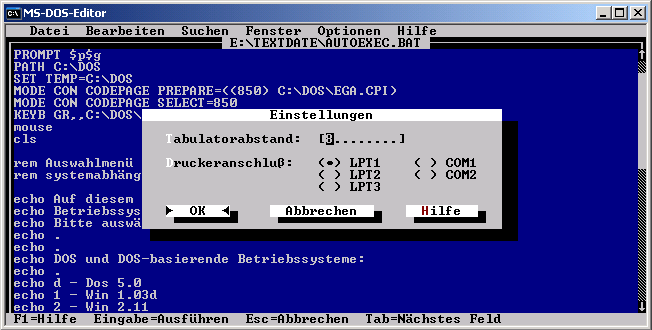
\includegraphics[scale=0.8]{imagens/EDIT_MSDOS}
    \\\textbf{Fonte: Internet Archive} \label{fig:EDIT_MSDOS}
\end{figure}
\FloatBarrier

Mais adiante na história, com o avanço das interfaces gráficas os editores de
texto passaram a se tornar mais visuais. É possível notar essa evolução em softwares
como o Notepad++ \cite{NotepadPlusPlus2025} até editores mais famosos como Visual
Studio Code \cite{VSCode2025} e o recente Zed \cite{ZedEditor2025}. Esses
editores de texto modernos oferecem uma ampla gama de recursos, como customização
e extensibilidade, suporte a plugins, integração com sistemas de controle de versão,
destacamento de sintaxe, autocompletar, entre outros, tornando a edição de texto
mais eficiente e produtiva.

O Notepad++ é um editor de texto de código aberto que se destaca por sua leveza e
simplicidade, oferecendo uma interface amigável e recursos avançados para edição
de código-fonte. Ele suporta várias linguagens de programação e possui recursos como
realceamento de sintaxe, autocompletar, busca avançada e suporte a plugins,
tornando-o uma escolha popular entre usuários que buscam um editor de texto
simples mas eficiente.

Por outro lado o Visual Studio Code é um editor de código-fonte desenvolvido
pela Microsoft que se tornou extremamente popular devido à sua extensibilidade e
integração com diversas ferramentas de desenvolvimento, além de oferecer uma ampla
gama de recursos como depuração integrada, controle de versão, suporte a várias linguagens
de programação e uma vasta biblioteca de extensões, permitindo que os usuários
personalizem sua experiência de edição de texto de acordo com suas necessidades.

\FloatBarrier

\begin{figure}[!htbp]
    \centering
    \caption{Visual Studio Code}
    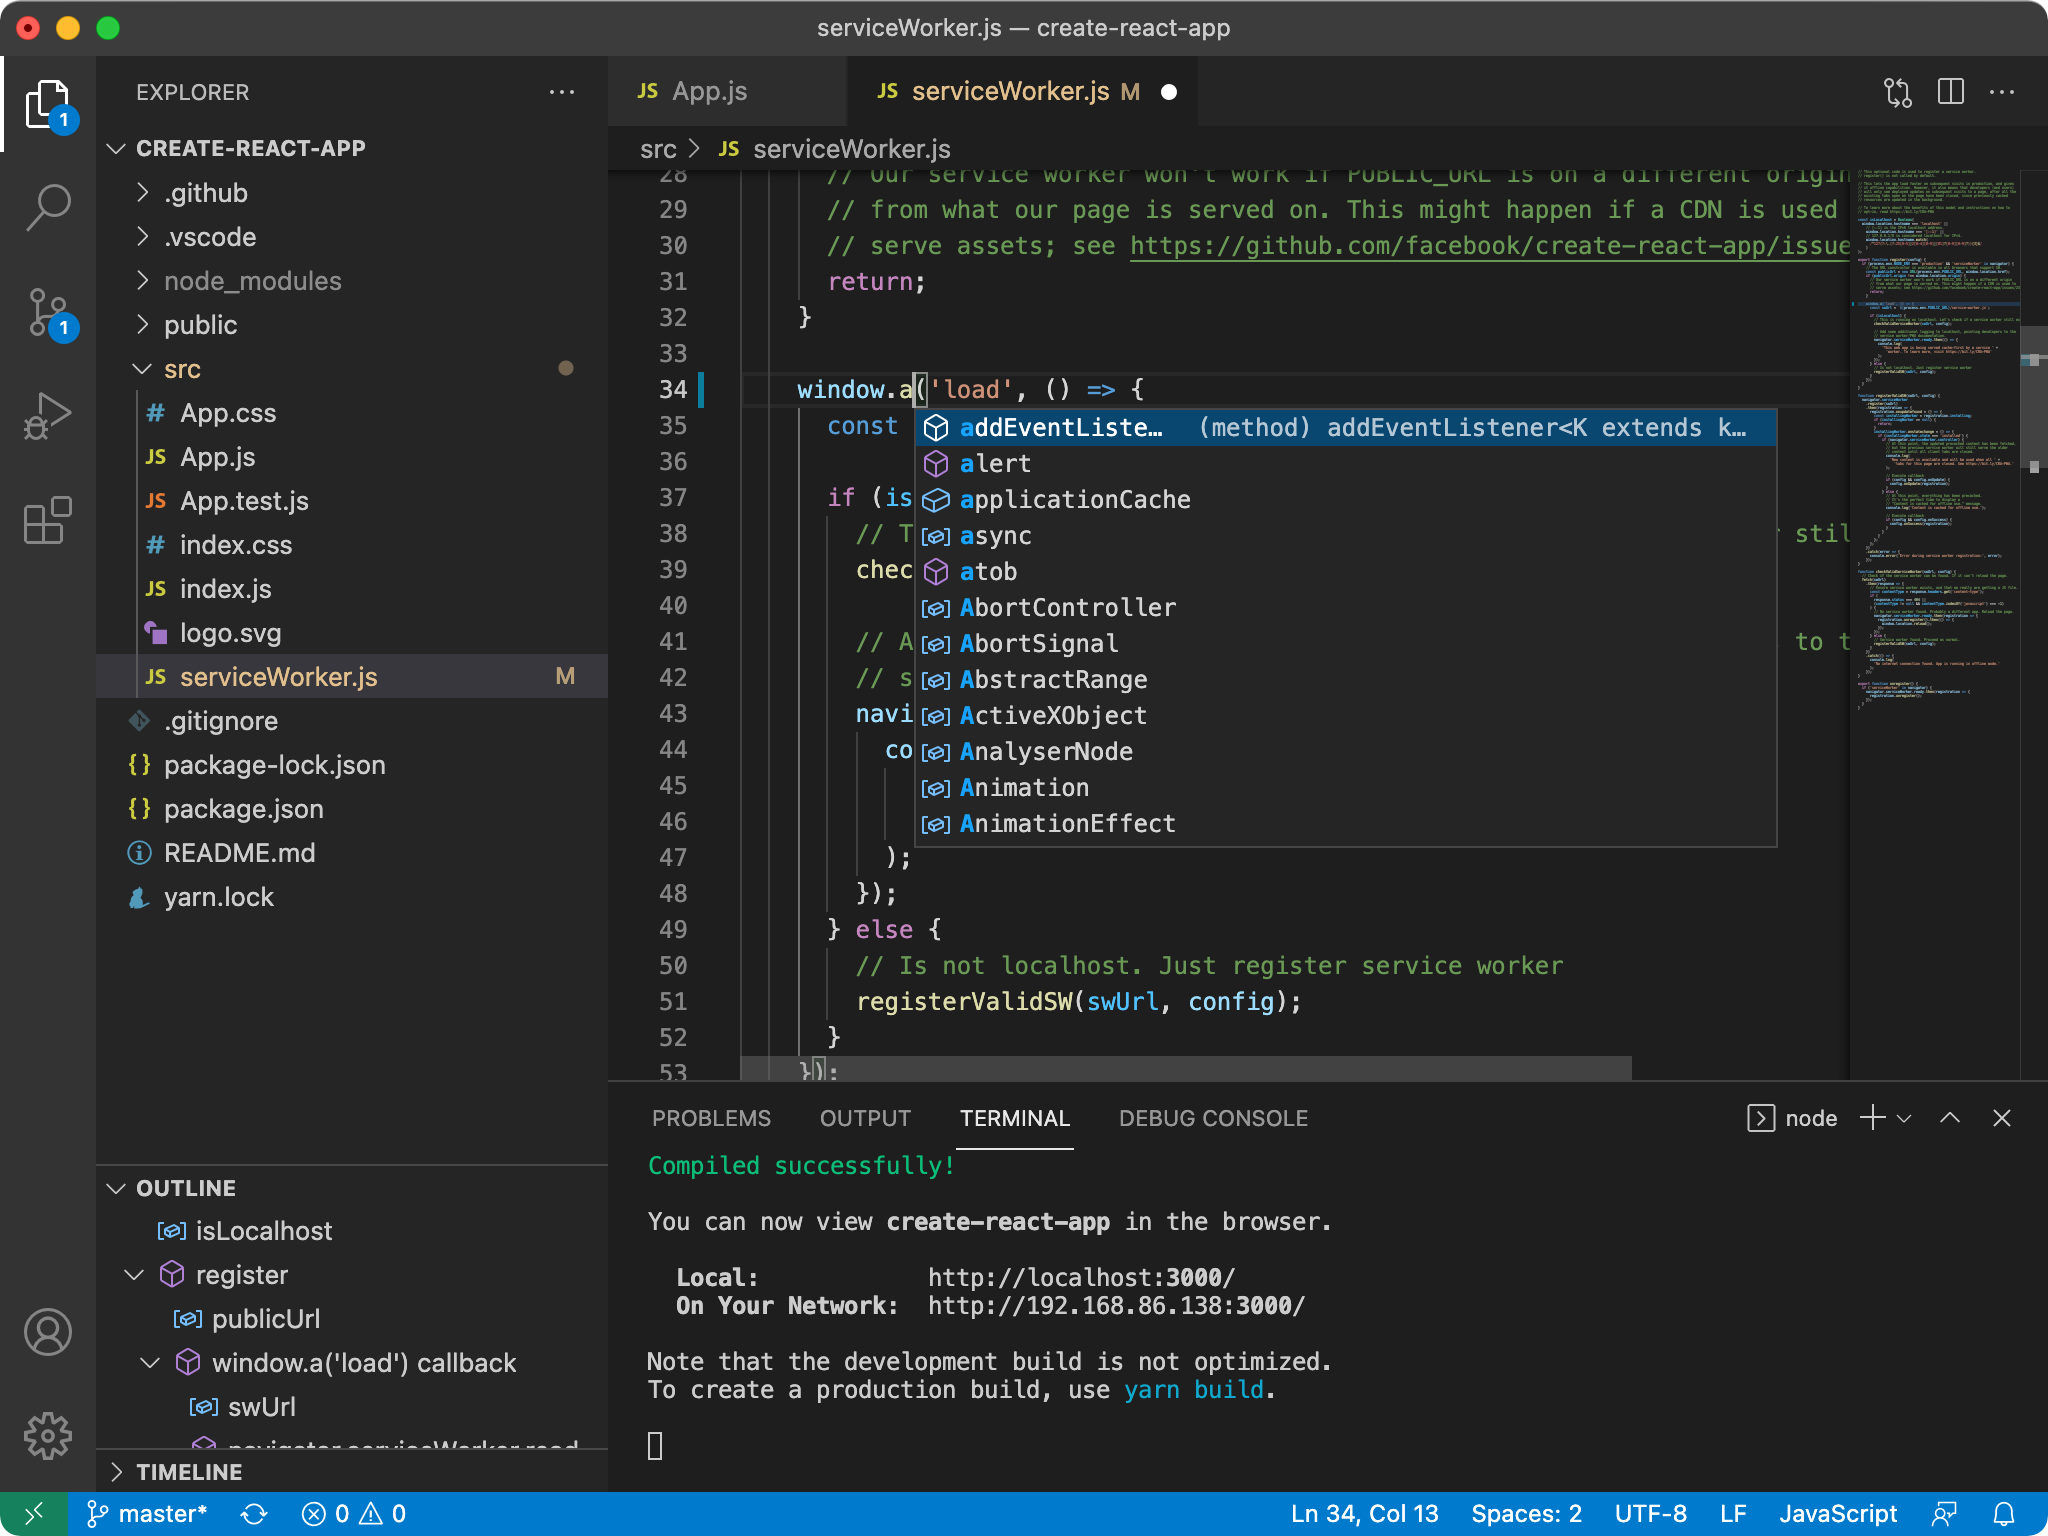
\includegraphics[scale=0.3]{imagens/VSCode}
    \\\textbf{Fonte: Github Microsoft - Visual Studio Code} \label{fig:VSCode}
\end{figure}
\FloatBarrier

Já o ainda em desenvolvimento Zed Editor se destaca por sua abordagem
colaborativa e em tempo real, permitindo que vários usuários editem o mesmo arquivo
simultaneamente. Ele oferece uma interface moderna e intuitiva e que se
assemelha muito ao Visual Studio Code, com recursos como realceamento de sintaxe,
autocompletar, integração com sistemas de controle de versão e suporte a plugins,
tornando-o uma escolha interessante para equipes de desenvolvimento que buscam
uma experiência de edição colaborativa e eficiente.

De modo geral, as interfaces podem ser divididas em dois grandes grupos: CLI e
GUI. Como apontados, as CLIs exigem um conhecimento técnico mais avançado, já que
utilizam constantemente de atalhos de teclado (ou do inglês, \textit{shortcuts}),
gerando uma curva de aprendizado mais íngreme, porém, com poder de controle
maior e fluidez na utilização diária, já que são interfaces altamente customizáveis
e cada usuário pode ter seu \textit{setup}. Por sua vez, as GUIs são mais
intuitivas por oferecerem elementos visuais como menus e ícones, facilitando o uso
e oferecendo experiência \textit{plug-and-play} (experiência de uso imediato), e
popularizando o computador como ferramenta pessoal.

Ainda hoje, após décadas de evolução, há usuários que preferem interagir por meio
de CLIs, como ao utilizar o editor NeoVim em sistemas UNIX. Com base nisso, este
trabalho propõe a criação de um editor CLI com uma interface mais moderna e
intuitiva, buscando unir o poder e a eficiência das CLIs à facilidade de uso presente
nas GUIs.

\section{Manipulação e Edição de Texto}

Portanto, no campo da computação, a existencia de ferramentas que lidam com a
manipulação e escrita de programas é, sem duvidas, essencial. Mas o mundo da edição
de texto é vasto e diversificado, abrangendo desde simples e comuns editores de
texto usados diariamente até sofisticados e completos ambientes de
desenvolvimento.

\subsection{Processadores de Texto}
\textbf{PROCESSADORES DE TEXTO: Microsoft Word, LibreOffice Writer, Google Docs,
etc.}

\subsection{Editores}

\textbf{EDITORES: Vi, Emacs, Nano, NeoVim, Visual Studio Code, Zed, Notepad++,
etc. Falar um pouco mais sobre como eles funcionam (já que já foram citados)}

\subsection{IDEs}

\textbf{IDEs: Visual Studio, CodeBlocks, NetBeans, IntelliJ IDEA, PyCharm, etc.}

\section{Principais Bibliotecas para Controle de Terminal em Linguagem C}

\textbf{MEIA PÁGINA PARA CADA BIBLIOTECA}

\textbf{Falar um pouco sobre cada uma e por que a escolhida foi a ncurses.}

\textbf{NCURSES e CURSES:}

\textbf{TERMBOX:}

\textbf{TERMINFO e TERMCAP:}

\textbf{S-LANG:}